\paragraph{Sats 3.11 (Bassatsen)} Låt $V$ vara planet eller rummet.
Om $f:V\rightarrow V$ är en linjär avbildning då är $f=f_{A}$, där
$A=\begin{pmatrix}
        \vline   &  & \vline    &  & \vline   \\
        f(e_{x}) &  & ff(e_{y}) &  & f(e_{z}) \\
        \vline   &  & \vline    &  & \vline
    \end{pmatrix}$.
\subparagraph{Bevis} Låt $\bm{v}\begin{pmatrix}
        v_{x} \\v_{y}\\v_{z}
    \end{pmatrix} =
    v_{x}e_{x}+v_{y}e_{y}+v_{z}e_{z}$.
Eftersom $f$ är linjär så får vi \\
\begin{center}
    $f(\bm{v})=f(v_{x}e_{x}+v_{y}e_{y}+v_{z}e_{z})=v_{x}f(e_{x})+v_{y}f(e_{y})+v_{z}+f(e_{z})=$ \\
    $\begin{pmatrix}
        f(e_{x}) &  & f(e_) &  & f(e_{z})
    \end{pmatrix}
    \begin{pmatrix}
        v_{x} \\v_{y}\\v_{z}
    \end{pmatrix}=A\bm{v} \blacksquare$
\end{center}


\paragraph{Sats 3.12} Varje linjär avbildning är en matrisavbildning och varje matrisavbildning är en linjär avbildning.

\section{Geometri hos linjära avbildningar (Avs 3.4)}
\paragraph{Proposition 3.14} Låt $f:V \rightarrow V$ vara en linjär avbildning och låt $L\subseteq V$ vara en linje.
Då är $f(L)$ en linje eller en punkt.\\
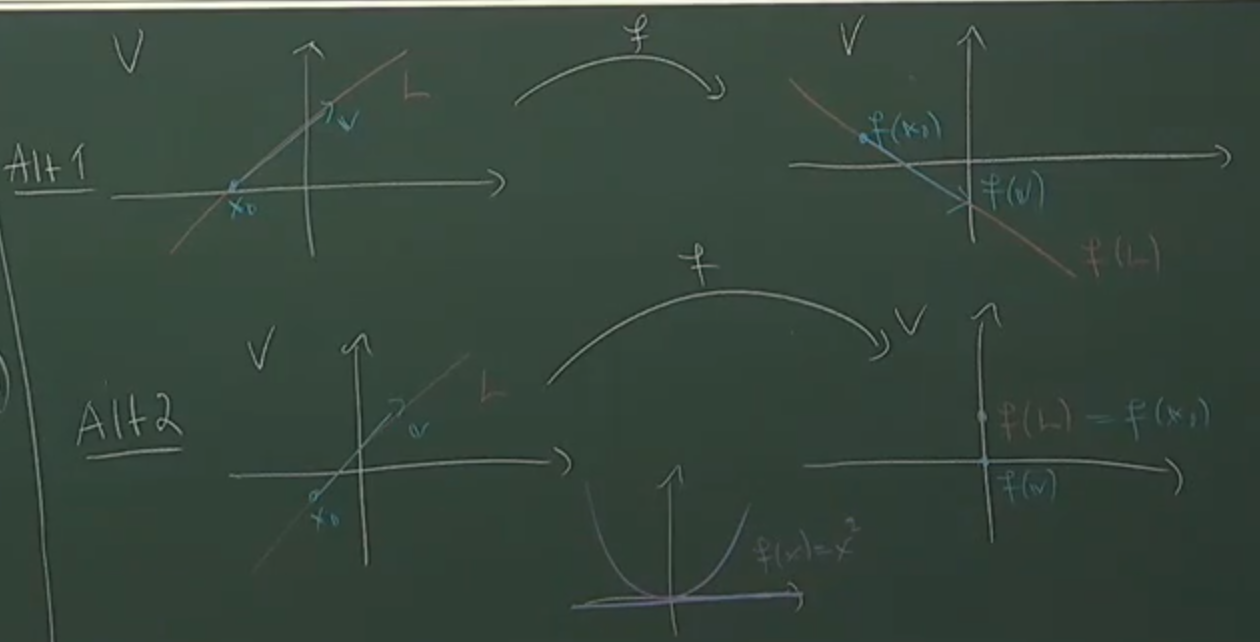
\includegraphics[scale=0.36]{imgs/img01.png}

\subparagraph{Bevis} Skriv linjen på formen $\bm{x}_{0}+t\bm{v}$.
Då ges $f(L)$ av alla punkter (vektorer) av $f(\bm{x}_{0}+t\bm{v})=f(\bm{x}_{0})+tf(\bm{v})$ vilket beskriver en linje om $f(\bm{v}\neq \bm{0})$.
Om $f(\bm{v})=\bm{0}$ då är $f(L)=f(\bm{x}_{0})$ $\blacksquare$

\paragraph{Proposition 3.16} Ortogonal projektion på en linje är en linjär avbildning.
\subparagraph{Bevis} Låt $\bm{r}$ vara en riktningsvektor för linjen.
För en allmän vektor $\bm{v}$ ges den ortogonala projektionen på $L$ av $f(\bm{v})=\frac{\bm{v}\cdot \bm{r}}{\bm{r}\cdot \bm{r}}\bm{r}$.
Visa nu att $f(\bm{u}+\bm{v})=f(\bm{u})+f(\bm{v})$ och $f(c\bm{v})>cf(\bm{v})$ $\blacksquare$

\paragraph{Ex} Låt $L$ vara en linje med riktningsvektor $\bm{r}=\begin{pmatrix}2\\3\end{pmatrix}$.
Bestäm matrisen för ortogonal projektion på $L$.
\subparagraph{Lösning} Matrisen ges av $A=\begin{pmatrix}f(e_{x})&f(e_{y})\end{pmatrix}$ där f är den otro. proj.p på $L$.
\begin{equation*}
    f(e_{x})=\frac{e_{x}\cdot \bm{r}}{\bm{r}\cdot \bm{r}}\bm{r}=\frac{\begin{pmatrix}1\\0\end{pmatrix}\cdot \begin{pmatrix}2\\3\end{pmatrix}}{\begin{pmatrix}2\\3\end{pmatrix}\cdot\begin{pmatrix}2\\3\end{pmatrix}}\begin{pmatrix}2\\3\end{pmatrix}=\frac{2}{13}\begin{pmatrix}2\\3\end{pmatrix}
\end{equation*}
\begin{equation*}
    f(e_{y})=\frac{e_{y}\cdot \bm{r}}{\bm{r} \cdot \bm{r}}\bm{r}=\frac{\begin{pmatrix}0\\1\end{pmatrix}\cdot \begin{pmatrix}2\\3\end{pmatrix}}{\begin{pmatrix}2\\3\end{pmatrix}\cdot\begin{pmatrix}2\\3\end{pmatrix}}\begin{pmatrix}2\\3\end{pmatrix}=\frac{3}{13}\begin{pmatrix}2\\3\end{pmatrix}
\end{equation*}

Alltså är $A=\begin{pmatrix}
    \vline&\vline\\
    f(e_{x})&f(e_{y})\\
    \vline&\vline
\end{pmatrix}=\frac{1}{13}\begin{pmatrix}
    2\cdot 2&3\cdot 2\\
    2\cdot 3&3\cdot 3
\end{pmatrix}=\frac{1}{13}\begin{pmatrix}4&6\\6&9\end{pmatrix}$
\begin{figure*}[h]
    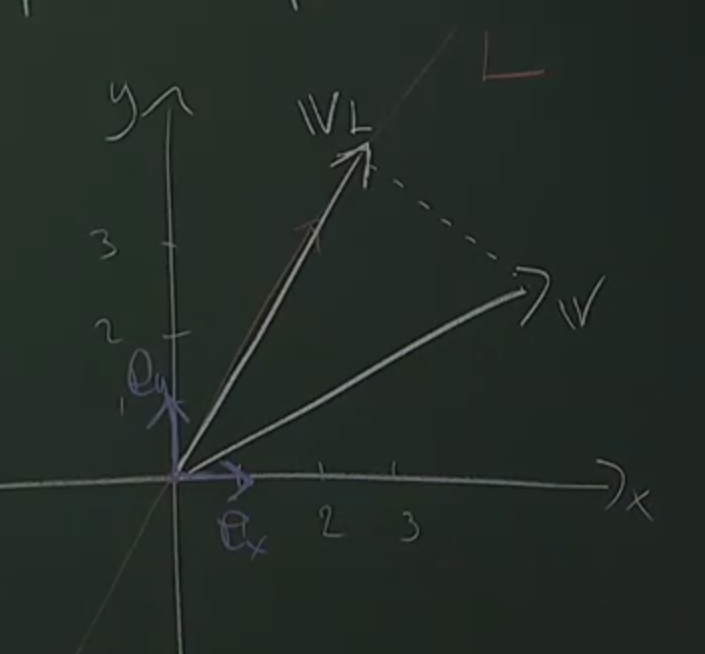
\includegraphics[scale=0.4]{imgs/img02.png}
\end{figure*}

\paragraph{Ex} Beskriv geometriskt vad $A=\begin{pmatrix}1&0\\0&0\end{pmatrix}$ är för linjär avbildning.
\subparagraph{Lösning} Låt $f$ vara den linjära avbildningen.
Då är $f(e_{x})=\begin{pmatrix}1\\0\end{pmatrix}=e_{x}$ och $f(e_{y})=\begin{pmatrix}0\\0\end{pmatrix}=\bm{0}$.
Detta är ortogonal projektion på x-axeln.\\
På sätt är $A=\begin{pmatrix}0&0\\0&1\end{pmatrix}$ ortogonal projektion på y-axeln och 
$B=\begin{pmatrix}0&0&0\\0&0&0\\0&0&1\end{pmatrix}$ är ortogonal projektion på z-axeln (i rummet).

\paragraph{Ex} Beskriv vilken linjär avbildning $a=\begin{pmatrix}0&1\\1&0\end{pmatrix}$ bestämmer.
\subparagraph{Lösning} Om $f$ är den linjära avbildningen så $f(e_{x})=\begin{pmatrix}0\\1\end{pmatrix}=e_{y}$
och $f(e_{y})=\begin{pmatrix}1\\0\end{pmatrix}=e_{x}$.
Så f byter  plats på basvektorerna.

\paragraph{Ex (Spegling)} Låt $L$ vara en linje med riktningsvektor $\bm{r}$ och genom origo.
\begin{figure*}
    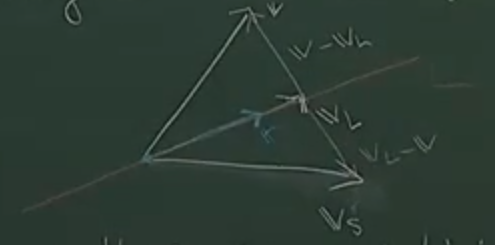
\includegraphics[scale=0.35]{imgs/img03.png}
\end{figure*}[h]
$\bm{v}_{s}$ är speglingen av $\bm{v}$ i linjen $L$.
$\bm{v}_{s}=\bm{v}_{L}+\bm{v}_{L}-\bm{v}=2\bm{v}_{L}-\bm{v}=2\frac{\bm{v}\cdot \bm{r}}{\bm{r}\cdot \bm{r}}\bm{r}-\bm{v}$.
Låt $\bm{r}=\begin{pmatrix}2\\3\end{pmatrix}$.
Då är 
\begin{equation*}
    (e_{x})_{s}=2\frac{e_{x}\cdot \bm{r}}{\bm{r}\cdot \bm{r}}\bm{r}-e_{x}=2\frac{4}{13}\begin{pmatrix}2\\3\end{pmatrix}-\begin{pmatrix}1\\0\end{pmatrix}=
    \frac{1}{13}(\begin{pmatrix}8\\12\end{pmatrix}-\begin{pmatrix}13\\0\end{pmatrix})=\frac{1}{13}\begin{pmatrix}-5\\12\end{pmatrix}
\end{equation*}
\begin{equation*}
    (e_{y})=2\frac{e_{y}\cdot \bm{r}}{\bm{r}\cdot \bm{r}}\bm{r} - e_{y}=2\frac{3}{13}\begin{pmatrix}2\\3\end{pmatrix}-\begin{pmatrix}0\\1\end{pmatrix}=
    \frac{1}{13}(\begin{pmatrix}12\\18\end{pmatrix}-\begin{pmatrix}0\\13\end{pmatrix})=\frac{1}{13}\begin{pmatrix}12\\5\end{pmatrix}
\end{equation*}
Matrisen för speglingen är $A_{s}=\frac{1}{13}\begin{pmatrix}-5&12\\12&5\end{pmatrix}$

\paragraph{Proposition 3.18} Rotation $\beta$ radianer moturs runt origo är en linjär avbildning vars matris ges av
$A=\begin{pmatrix}
    cos\beta & -sin\beta\\sin\beta & cos\beta
\end{pmatrix}$
\subparagraph{} Beviset använder additionsformlerna för de trigonometriska funktionerna.

\paragraph{Ex} Låt $f$ vara rotation $\frac{\pi}{4}$ moturs runt origo.
Beräkna matrisen till $f$.
\subparagraph{Lösning} 
\begin{figure*}[h]
    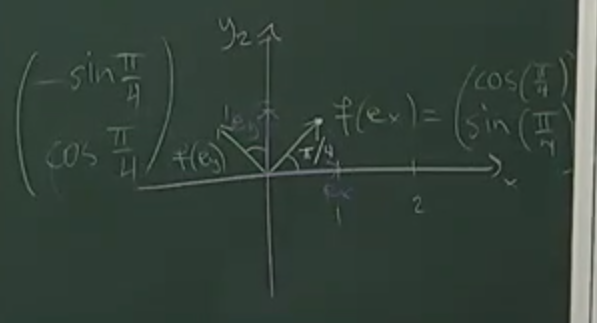
\includegraphics[scale=0.3]{imgs/img04.png}
\end{figure*}
Matrisen ges av $\begin{pmatrix}
    cos(\frac{\pi}{4}) & -sin(\frac{\pi}{4})\\sin(\frac{\pi}{4}) & cos(\frac{\pi}{4})
\end{pmatrix}$

\chapter{Sammansatta avbildningar (Avs 3.5)}
\paragraph{Proposition 3.22} Låt $f:V\rightarrow W$ och $g:W\rightarrow V$ vara linjära avbildningar som ges $A$ respektive $B$.
Då är $fog:W\rightarrow W$ och $gof:V\rightarrow V$ linjära avbildningar med matriser $AB$ respektive $BA$.\\
Eftersom vi vet att i allmänhet så är $AB\neq BA$ och därför är $fog\neq gof$.\\
Till exempel är resultatet inte samma om vi roterar och sen projicerar som om vi projicerar och sedan roterar.

\paragraph{Proposition 3.26} Låt $f:V\rightarrow V$ vara en linjär avbildning med matris $A$.\\
Då är $f$ inverterbar om och endast om $A$ är inverterbar.\\
Om $f$ är inverterbar då är $f^{-1}$ linjär och dess matris är $A^{-1}$.

\paragraph{Ex} Rotation är en inverterbar linjär avbildning.
\subparagraph{Bevis} Rotation $\beta$ radianer moturs ges av $A=\begin{pmatrix}cos\beta & -sin\beta\\sin\beta & cos\beta\end{pmatrix}$.
\begin{equation*}
    det(A)=cos^{2}\beta + sin^{2}\beta=1\neq 0
\end{equation*}
Därför är $A$ inverterbar och alltså är rotation inverterbar.
\begin{equation*}
    a^{1}=\begin{pmatrix}
        cos\beta&sin\beta\\-sin\beta&cos\beta
    \end{pmatrix}=\begin{pmatrix}
        cos(-\beta)&-sin(-\beta)\\sin(-\beta)&cos(-\beta)
    \end{pmatrix}
\end{equation*}